%
%  monografia
%
%  Created by Ricardo de Cillo on 2012-05-27.
%  Copyright (c) 2012 __MyCompanyName__. All rights reserved.
%
\documentclass[a4paper,11pt]{article}

% Use utf-8 encoding for foreign characters
\usepackage[brazil]{babel}
\usepackage[utf8]{inputenc}
\usepackage[T1]{fontenc}

% Setup for fullpage use
\usepackage{fullpage}
\usepackage{setspace}

% Uncomment some of the following if you use the features
%
% Running Headers and footers
%\usepackage{fancyhdr}

% Multipart figures
%\usepackage{subfigure}

% More symbols
\usepackage{amsfonts}
\usepackage{amssymb, amsmath}
%\usepackage{latexsym}

% Surround parts of graphics with box
\usepackage{boxedminipage}

% Package for including code in the document
\usepackage{listings}

% If you want to generate a toc for each chapter (use with book)
\usepackage{minitoc}

% This is now the recommended way for checking for PDFLaTeX:
\usepackage{ifpdf}

%\newif\ifpdf
%\ifx\pdfoutput\undefined
%\pdffalse % we are not running PDFLaTeX
%\else
%\pdfoutput=1 % we are running PDFLaTeX
%\pdftrue
%\fi

\ifpdf
\usepackage[pdftex]{graphicx}
\else
\usepackage{graphicx}
\fi


\usepackage{xcolor}
\newcommand{\TODO}[1]{\textcolor{red}{#1}}


%% \title{Aplicação de análise morfológica para segmentação de páginas em imagens de documentos}
%% \author{ Aluno: Ricardo de Cillo \\ Supervisora: Nina S. T. Hirata }

% \date{2012-05-27}

\begin{document}

%  \maketitle

% =======================================================================
% CAPA
% =======================================================================

\thispagestyle{empty}
\

\

\

\

\begin{center}
{\bf \Large Trabalho de Formatura Supervisionado}

\bigskip
\bigskip
{\bf \LARGE Aplicação de análise morfológica para segmentação de páginas em imagens de documentos}

\bigskip
{\large Ricardo de Cillo}

\bigskip
Supervisora: Nina S. T. Hirata 

\bigskip
Departamento de Ciência da Computação\\
Intituto de Matemática e Estatística, IME-USP
\end{center}


\bigskip
\begin{quote}
\begin{spacing}{1.2}
\noindent {\bf \large Resumo}: Neste texto apresentamos nosso estudo sobre a aplicação de operadores morfológicos à segmentação de páginas de documentos, etapa importante na análise de documentos que busca extrair informações sobre a sua estrutura: regiões com títulos, legendas, figuras e blocos de texto. A qualidade da solução obtida será medida e comparada, segundo os mesmo critérios aplicados à resultados considerados estado da arte por pesquisadores da área.
\end{spacing} 
\end{quote}

\bigskip
\begin{center}
São Paulo, \today
\end{center}


\newpage

\tableofcontents

\newpage
\setcounter{page}{1}

\section{Introdução}

Processamento e análise de documentos é uma importante subárea da área
de reconhecimento de padrões cujo principal objetivo é a
interpretação de um documento, ou seja, o entendimento
da sua estrutura bem como o reconhecimento de cada um dos
componentes estruturais.

\begin{figure*}[htb]
\begin{center}
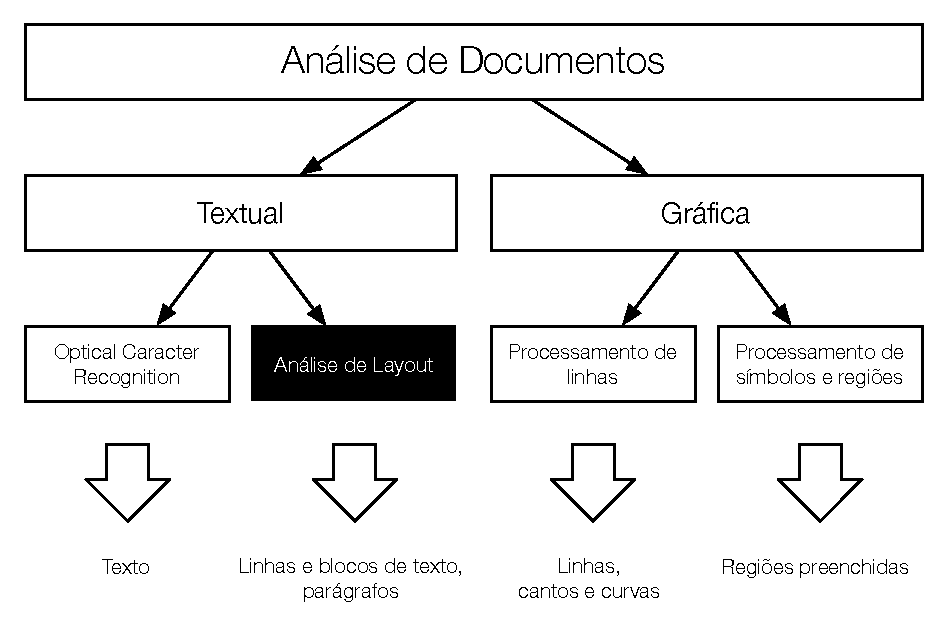
\includegraphics[width=0.7\textwidth]{assets/document_processing_areas_hierarquies.pdf}
\end{center}
\caption{Contextualização do tema do trabalho entre as áreas da
  análise de documentos. Adaptado de~\cite{Kasturi_OGorman_Govindaraju_2002}.}
\label{fig:context1}
\end{figure*}

Segmentação de página refere-se à tarefa de separar e rotular os diferentes
componentes que fazem parte da estrutura das páginas de um
documento, tais como: blocos de texto, gráficos, figuras, títulos,
legendas, separadores, tabelas, fórmulas matemáticas e regiões com
ruído.

Em geral, a segmentação de página é um dos primeiros passos no
processo de entendimento de um documento. Uma vez identificiados os
blocos estruturais, processamentos específicos para cada tipo de bloco
podem ser aplicados. Por exemplo, no caso de blocos de textos é
conveniente fazer o reconhecimento de texto para que o mesmo possa ser
armazenado em formato texto (e não imagem). Por outro lado, no caso de
imagens, pode ser interessante armazená-las em alta resolução para
manter a qualidade. Documentos digitalizados podem ser processados
eficientemente em processos que envolvem armazenamento, edição,
transmissão, ou busca, por exemplo.

Devido à grande quantidade de documentos, é interessante que o seu
processamento seja realizado de forma automatizada ou pelo menos
semi-automatizada. Para tal, diversas soluções computacionais vêm
sendo propostas para o problema ao longo dos anos desde o surgimento
desse campo de pesquisa. Automatizar esta tarefa reduz custos, aumenta
a velocidade e capacidade de processamento de documentos além de
possivelmente reduzir a taxa de erro humano na classificação de uma
região.

Neste trabalho exploraremos a aplicabilidade de operadores
morfológicos automaticamente gerados ao problema de segmentação de
páginas.

\TODO{completar a descrição da estrutura do texto}

Este texto está organizado da seguinte forma. Na seção~\ref{sec:fundamentos},
apresentamos as definições e conceitos básicos que serão importantes
para a leitura deste texto.

\section{Fundamentos}
\label{sec:fundamentos}

\subsection{Imagens digitais}
  Uma imagem digital monocromática pode ser definida como uma função $f:
  \mathbb{E} \subset \mathbb{Z}^2 \to \mathbb{K} = \{0,1,\ldots,k-1\}$, na qual $k$ representa o número de tons de cinza. Tipicamente adota-se $k=256$, ou seja, 8-bits de cor. Quando $k=1$ as imagens são denominadas {\bf binárias}; quando $k>1$ as imagens são denominadas {\bf tons de cinza}. Na prática, o domínio $\mathbb{E}$ é um retângulo finito de dimensões $m\times n$ (uma matriz de $m$ linhas e $n$ colunas).

  Uma imagem RGB (colorida) é uma função $f: \mathbb{E} \to \mathbb{K}^3$, onde cada componente $\mathbb{K}$ representa a intensidade das cores vermelho, verde e azul, respectivamente.

\subsection{Operadores de imagens}
Um operador de imagens é uma função que mapeia imagens em
imagens. Denotando $\mathbb{E}=\mathbb{Z}^2$, $K=\{0,1,\ldots,k-1\}$ e
todas as imagens definidas em $\mathbb{E}$ por $K^{\mathbb{E}}$,
  podemos representar um operador de imagens como $\Psi: K^{\mathbb{E}}
    \to K^{\mathbb{E}}$.

\subsubsection{Binarização de imagens}

A classe de operadores estudada restringe-se ao domínio das imagens binárias. Porém as imagens obtidas através de digitalização usualmente são coloridas (RGB de 24-bits). O processo de binarização é realizado por um operador que mapeia uma imagem colorida ou monocromática em uma imagem binária.

Neste trabalho, primeiramente transformamos as imagens coloridas para níveis de cinza e posteriormente aplicamos a binarização.

Existem muitos algoritmos que realizam esta tarefa. Uma revisão extensa dos mais conhecidos métodos de binarização é apresentada em \cite{citeulike:890354}. Todos eles se aplicam a imagens em níveis de cinza, portanto inicialmente transformaremos a imagem colorida $f$ em níveis de cinza $g$:

\begin{equation}
  f(x) \in \mathbb{K}^3 \rightsquigarrow g(x) \in \mathbb{K} \rightsquigarrow b(x) \in \{0, 1\}
\end{equation}

\subsection{Classificação de objetos}

Na área de reconhecimento de padrões e aprendizado computacional
estudam-se métodos e técnicas para classificação de dados em geral. Os
dados (padrões) a serem classificados correspondem, em geral, à
representação digital de algum objeto concreto ou abstrato. O objetivo
da classificação é atribuir um rótulo de classe a cada padrão
observado.

Dependendo do problema, os rótulos de classe podem ser conhecidos ou
não. Por exemplo, se desejamos fazer o reconhecimento de caracteres,
os padrões são a imagem dos caracteres e os rótulos de classe são as
identificações dos possíveis caracteres. Por outro lado, em problemas
como na classificação de perfil de consumidores, pode não haver um
conjunto de perfis pré-estabelecidos e o objetivo seria então
identificar a possível existência de perfis. O primeiro é conhecido
como problema de classificação supervisionada e o segundo como
classificação não-supervisionada.

No caso da classificação supervisionada, supõe-se que os padrões são
elementos de um espaço $X$ e que o conjunto de rótulo de classe é dado
por $Y=\{y_1,y_2,\ldots,y_c\}$. Assim, um classificador pode ser
expresso por uma função $f: X \to Y$.

Frequentemente $X$ é um subespaço de $\mathbb{R}^d$. Assim, um padrão
é representado por uma $d$-upla $\mathbf{x}=(x_1,x_2,\ldots,x_d) \in
\mathbb{R}^d$.

\subsection{Segmentação de imagens}

A segmentação de imagens é um processamento comum a praticamente
todos os processos que envolvem análise de imagens. Segmentar uma
imagem corresponde a particionar o seu domínio, de forma que cada
região resultante corresponda (do ponto de vista semântico) a uma
componente de interesse na análise em questão. Este problema pode ser modelado como uma classificação de objetos, onde o conjunto de pixels de uma imagem são os objetos em $X$ e as componentes em $Y$ são regiões de interesse, como ilustrado na tabela \ref{tab:image_segmentation}.

\begin{table}
  \caption{Exemplo de segmentação de imagem: separando frente e fundo.}
  \begin{tabular}[p]{@{}ccc@{}}
    \centering
    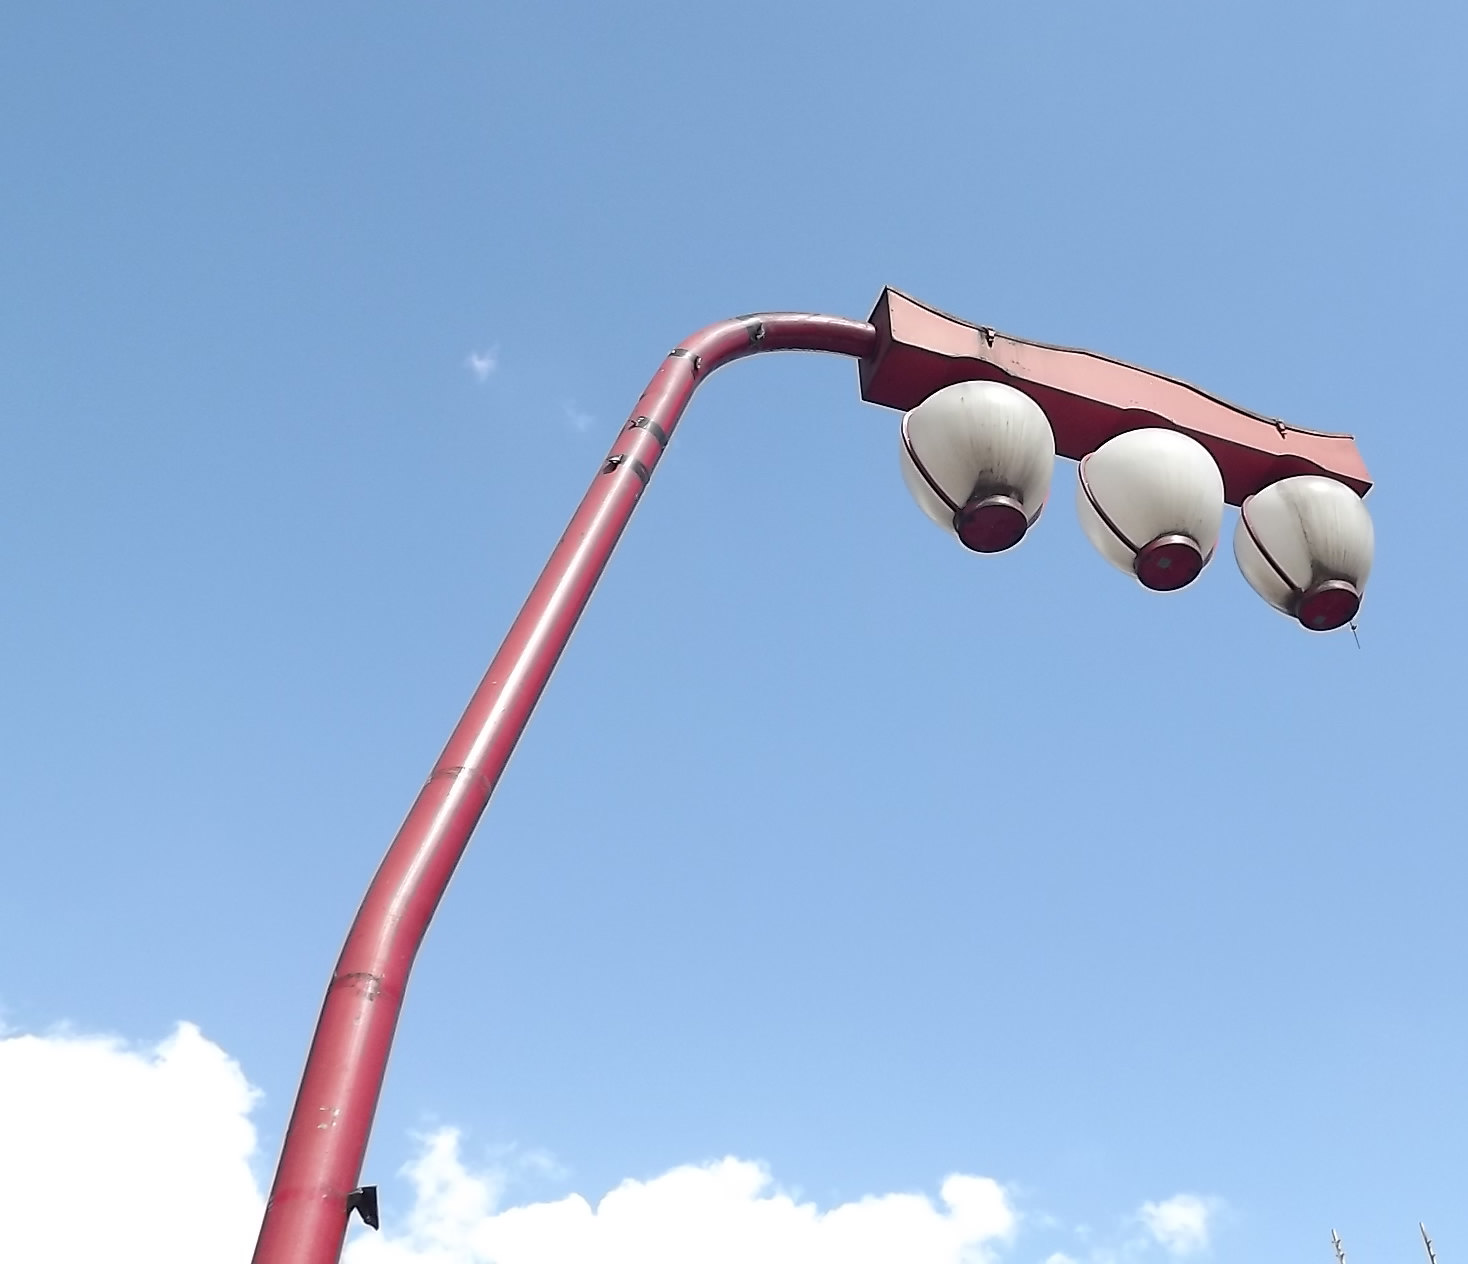
\includegraphics[width=0.3\textwidth]{assets/image_segmentation/classification_example.png}
    &
    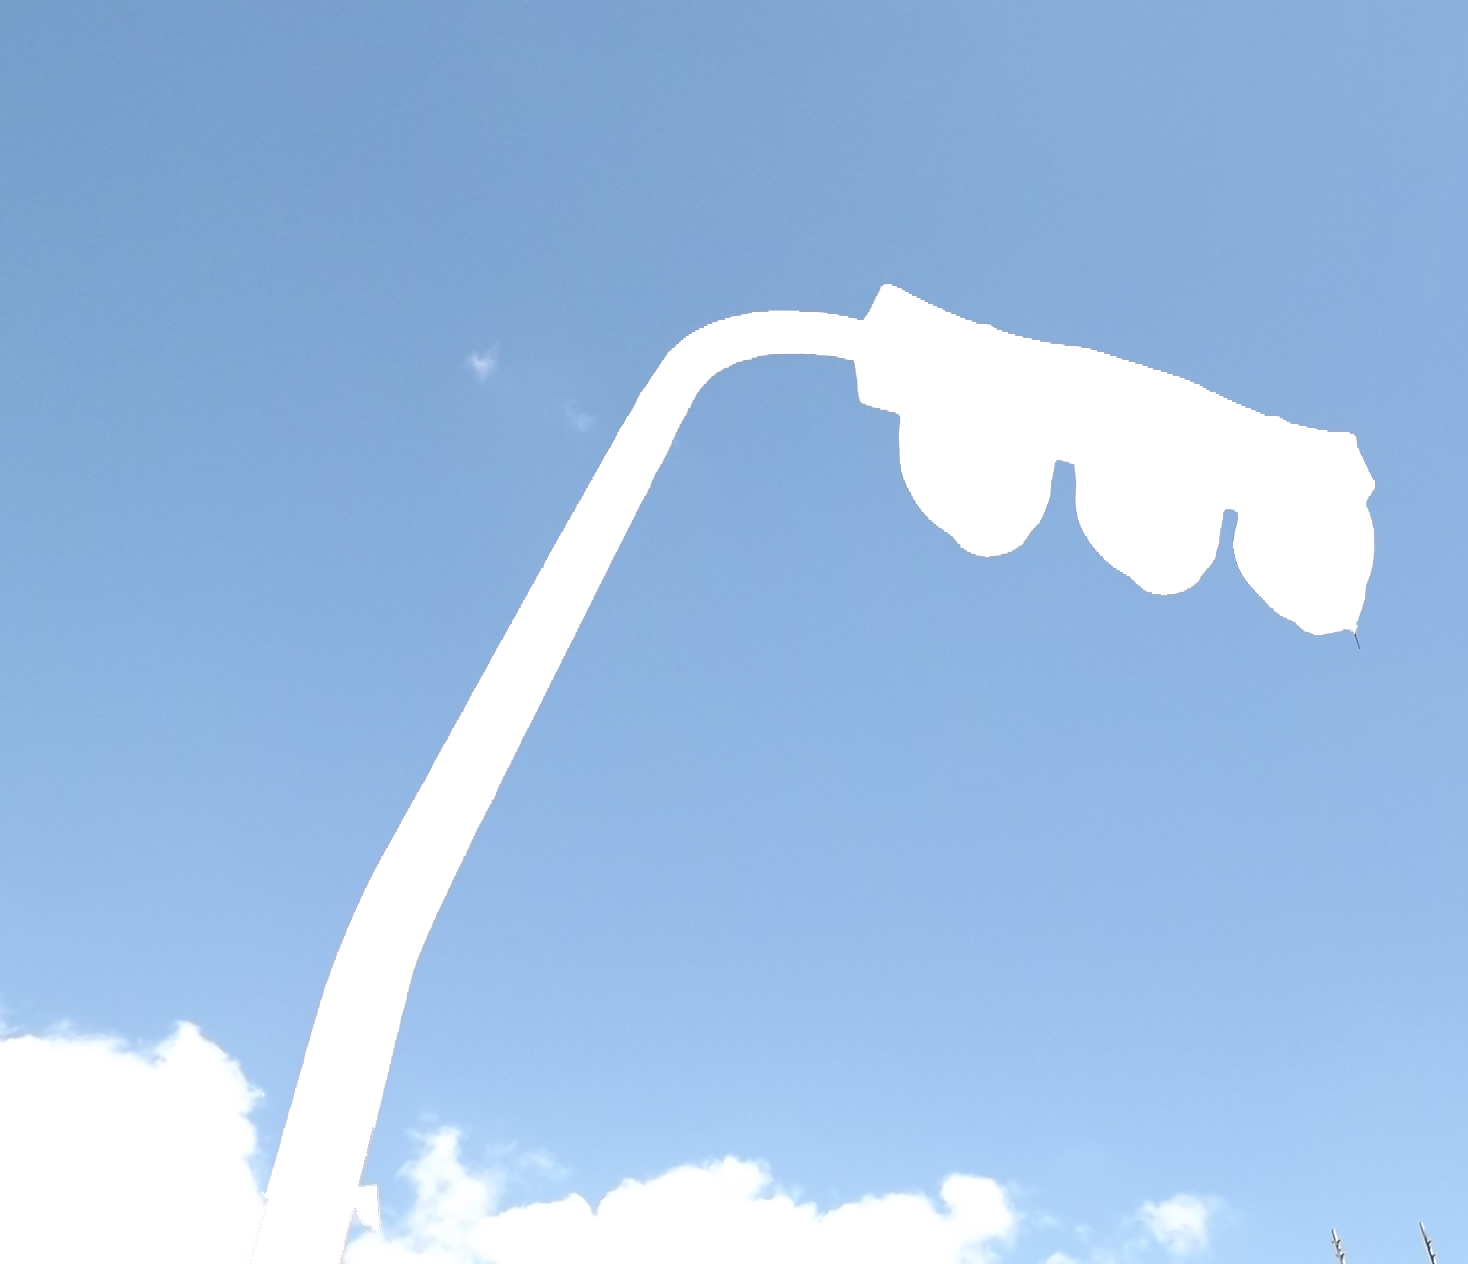
\includegraphics[width=0.3\textwidth]{assets/image_segmentation/background.png}
    &
    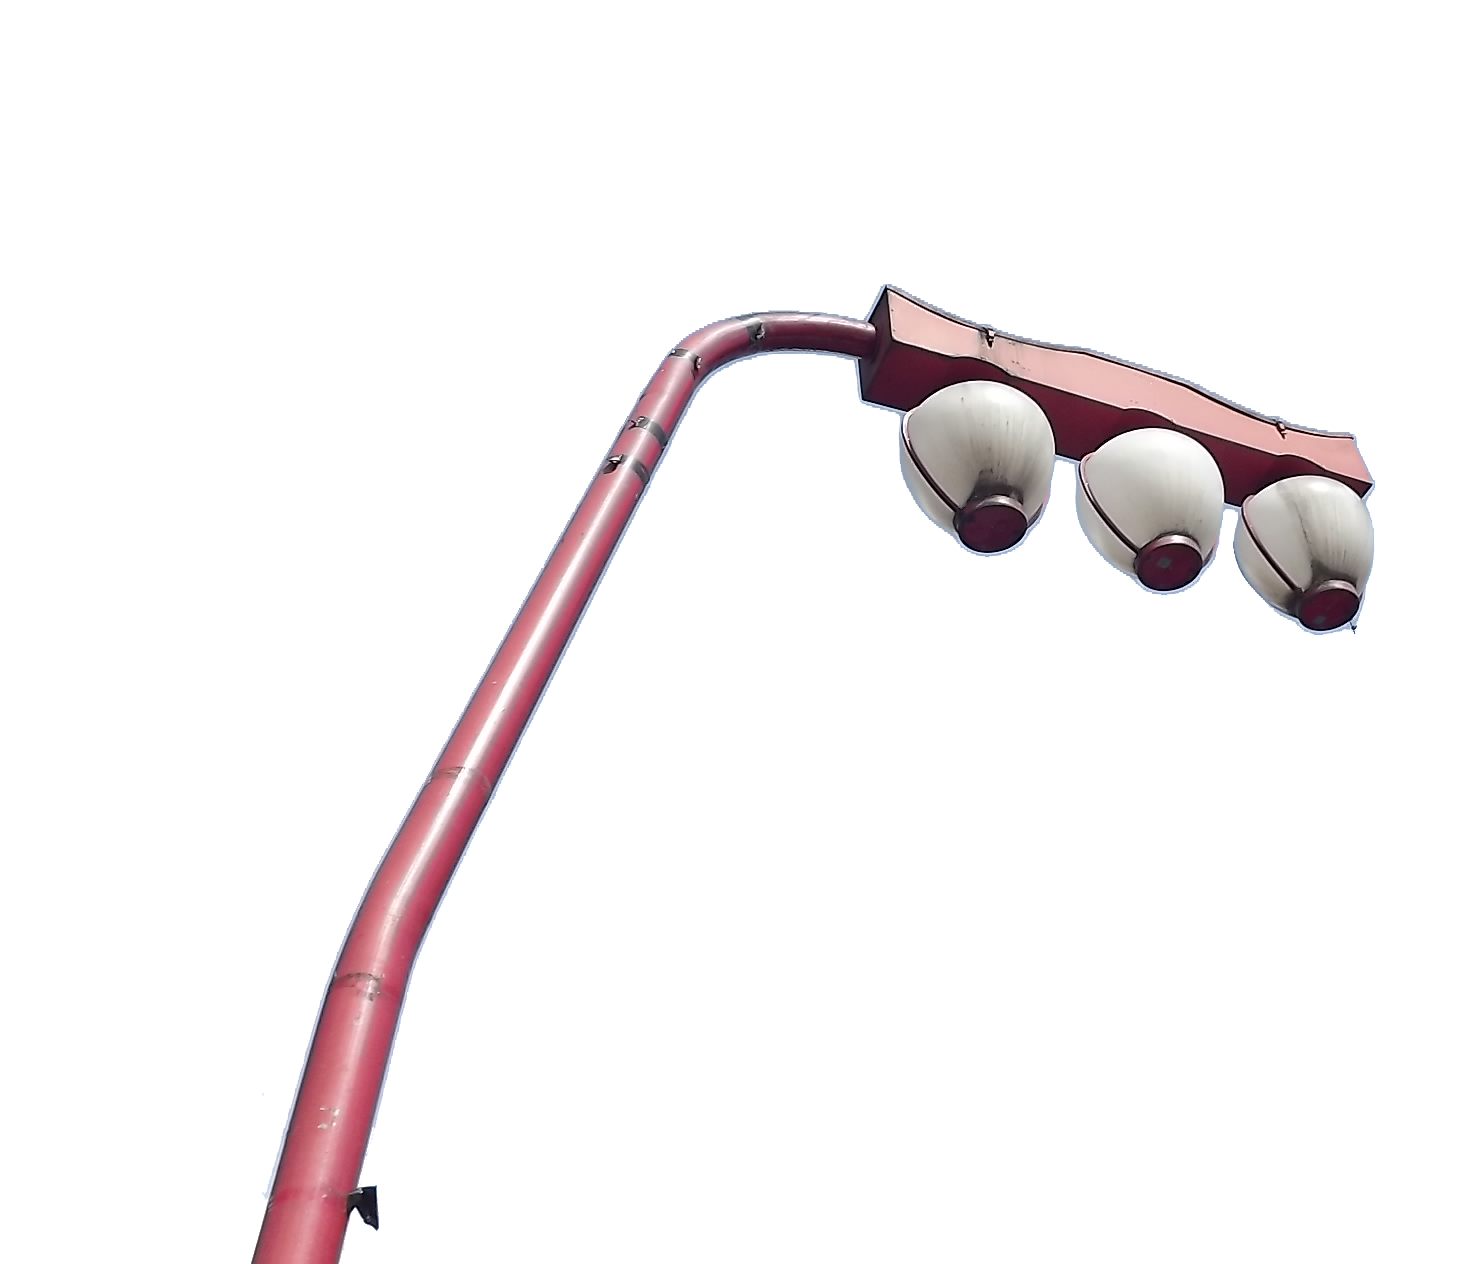
\includegraphics[width=0.3\textwidth]{assets/image_segmentation/foreground.png}

    \\

    imagem original
    &
    fundo
    &
    frente

    \label{tab:image_segmentation}
  \end{tabular}
\end{table}

\subsection{Classificação dos componentes}
\label{sec:components}

O problema de segmentação de imagens de documentos pode ser modelado como um problema de classificação de objetos, onde cada pixel da imagem é rotulado através de uma função classificadora

\begin{equation}
\Psi \colon \mathbb{E} \rightarrow \mathbb{Y}
\end{equation}

sendo $\mathbb{Y}$ um conjunto composto pelas regiões de interesse:

\begin{itemize}
  \item blocos de texto: região com parágrafos
  \item gráficos
  \item figuras
  \item títulos
  \item legendas
  \item separadores
  \item tabelas
  \item fórmulas matemáticas
  \item regiões com ruído
\end{itemize}

\subsection{Avaliação da segmentação}

\TODO{Dizer aqui como se avalia uma segmentação. Poderia ser a nível
  de pixel, ou a nivel de regiões ou componentes. Pixel é fácil, mas
  tem os potenciais problemas. No caso de região é preciso definir
  como comparar regiões --- caso dos polígonos isotéticos, etc etc}

Os dois principais métodos utilizados para avaliar a qualidade das soluções para este problema são a comparação da classificação dos pixels individualmente ou a classificação de regiões.
Optamos pela comparação entre pixels pois nosso método produz como resultado a classificação de pixels e não a delimitação de regiões. Seria necessário agrupar os pixels em regiões para que pudéssemos realizar outros tipo de avaliação, o que foge ao escopo deste trabalho.

Uma vantagem na comparação entre pixels e não regiões é o fato de que evitamos restrições arbitrárias na forma das regiões.


\section{Aprendizado de operadores morfológicos}

Construir operadores morfológicos que resolvam problemas complexos como o de segmentar uma página de documento, pode ser uma tarefa que demande muito tempo, experiência e conhecimento específico do assunto. Como estas imagens possuem características distintas dependendo da publicação, é possível que apenas um operador não consiga ser aplicado a todas as imagens. Ou seja, construir operadores com facilidade é um fator sensível para a escolha desta abordagem.

Nesta seção apresentamos um método para projetar operadores morfológicos de forma automática utilizando tecnicas de aprendizado computacional. Primeiramente definiremos o conceito de operadores morfológicos.

\subsection{Operadores morfológicos binários}

Informalmente, operadores morfológicos são transformações entre imagens binárias que podem ser descritas através de propriedades geométricas e topológicas. Um exemplo amplamente conhecido é o da  dilatação, cuja aplicação está exemplificada na figura \TODO{ref}.

\TODO{figura com dilatação e erosão}

Formalmente define-se um operador morfológico binário como uma transformação localmente definida e invariante por translação entre reticulados completos.

Um dos principais resultados da morfologia matemática revela que qualquer operador binário pode ser decomposto em uma combinação de operadores mais simples, dilatação \eqref{eq:dilatacao} e erosão \eqref{eq:erosao}, chamados de elementares.

\begin{equation}
  \label{eq:dilatacao}
  \delta_{B}(X) = \{ x \in E \colon B_{x} \cap X \neq \emptyset \}
\end{equation}

\begin{equation}
  \label{eq:erosao}
  \varepsilon_{B}(X) = \{ x \in E \colon B_{x} \subseteq E \}
\end{equation}

O conjunto $B$ é denominado elemento estruturante.

\subsection{Treinamento}

A fim de projetar operadores morfológicos complexos de forma automática, utilizaremos o método proposto em \TODO{ref}. Nele, um conjunto de pares de imagens de treinamento é transformado em um operador. Estes pares são compostos da imagem \textbf{original}, denotada por $X$ e sua \textbf{derivada} $Y$, que exemplifica a transformação desejada. (figura \TODO{ref}).

O processo consiste de 3 etapas (diagrama \TODO{ref}): coleta, decisão e minimização. Ao fim, teremos uma função booleana que aproxima é uma aproximação do operador desejado. A seguir detalhamos cada uma das etapas.

\subsubsection{Coleta}

Seja $C(X_W) = \{X \cap W + z \colon z \in E \}$ o conjunto de todas as configurações observadas ao se transladar a janela $W$ sobre a imagem $X$. Seja $Y_z$ o valor 0 ou 1 encontrado na imagem $Y$ na posição $z$. Construimos uma tabela com três colunas: $C(X_W)$, frequência observada $Y_z = 0$ e frequência $Y_z = 1$. (tabela exemplo \TODO{ref})

\subsubsection{Decisão}

As configurações observadas na etapa anterior possuirão valores relacionados em $Y$ iguais a 0, 1 ou ambos. No caso de tanto 1 como 0 terem sido observados, escolheremos como valor para a função final a com maior número de ocorrências. No caso de alguma configuração não ter sido observada ou de o número de ocorrências empatar, escolheremos o valor que simplifica a próxima etapa: minimização.

\subsubsection{Minimização}

\TODO{Descrever algoritmo ISI}

\section{Metodologia}

O método proposto é baseado em operadores morfológicos automaticamente gerados, ou seja, construímos um segmentador genérico a partir de alguns exemplos de segmentação (pares de imagens). A seguir detalhamos cada uma das etapas envolvidas.

    \begin{enumerate}
      \item Preparação das imagens de treinamento
      \item Construção dos operadores
      \item Aplicação dos operadores
      \item Consensualização
    \end{enumerate}

    \subsection{Preparação das imagens de treinamento}

      O primeiro passo consiste na produção dos pares de imagens de treinamento. Estes pares consistem da imagem original binarizada e de sua variante segmentada.

      Para cada imagem original geramos $n$ pares de exemplo, sendo $n$ o número de tipos de regiões que desejamos segmentar. No caso deste trabalho nos limitamos a três: texto, título e citação.

      A variante segmentada pode ser obtida através de duas estratégias: preservação ou preenchimento da região de interesse. A imagem *exemplos de treinamento* ilustra a geração das imagens de exemplos usando as duas estratégias.

      \TODO{*exemplos de treinamento*}

      \TODO{Falar sobre binarização em uma seção sobre o dataset e pré-processamentos}

    \subsection{Construção dos operadores}

      O algoritmo gerador de operadores morfológicos recebe como entrada um conjunto de pares de imagens de exemplo do passo anterior. Treinamos um operador para cada tipo de região utilizando a biblioteca TRIOS \TODO{ref}. Os parâmetros para o treinamento foram ajustados experimentalmente \TODO{ref experimentos}.

      \TODO{Imagem com 2 a 3 pares de exemplos de segmentação de texto para treinamento de um operador}

    \subsection{Aplicação dos operadores}

      Construidos os operadores para cada tipo de região, aplicamos todos os operadores às imagens que desejamos segmentar obtendo um resultado para cada operador. Sendo $n$ operadores e $m$ imagens, obtemos $nm$ resultados.

      \TODO{exemplo de aplicação de $n$ operadores}

    \subsection{Consensualização}

      A aplicação de operadores diferentes à mesma imagem pode gerar resultados incoerentes. Pixels classificados como pertencentes a mais de uma região fazem com que a união dos resultados seja impossível sem nenhum tipo de processamento. Para concluirmos a segmentação é necessário chegar a um consenso sobre qual operador possui a maior probabilidade de estar certo a cada pixel de classificação conflitante.

      Partindo da observação de que pixel pertencente a uma certa região costuma estar cercados por pixels da mesma região, aplicamos um processo de escolha por maior contagem de pixels na vizinhança. Ou seja, se houver um conflito de classificação de um pixel entre texto ou título, conta-se quantos pixels na vizinhança pertencem a uma dada região e a que obtiver maior contagem ganha.

      \TODO{Exemplo de conflito e contagem para consenso}

\section{Experimentos}

  Realizamos experimentos com diferentes publicações, quantidade de regiões, quantidade de imagens de treinamento, diferentes parâmetros do TRIOS como tamanhos e formas de janela, e tamanhos de janelas na etapa de consensualização.

  \subsection{Agrupamento de publicações}

    Neste experimento medimos o desempenho do método quando aplicado a conjuntos de imagens de publicações diferentes ou apenas de uma única publicação. Diferentes publicações possuem diferentes tipos de regiões, utilizam famílias de fontes e tamanhos diferentes.

    \begin{itemize}
      \item CACM
      \item FORTUNE
      \item IEEE
      \item TIME
      \item MIX
    \end{itemize}

    \TODO{mostra imagens de revistas com fontes bem diferentes}

  \subsection{Quantidade de imagens de treinamento}

    Medimos a sensibilidade do método à quantidade de imagens de treinamento. Analisamos separadamente a redução na taxa de erro de classificação por tipo de região.

    \begin{itemize}
      \item 1/3
      \item 2/3
      \item full
    \end{itemize}

  \subsection{Tamanho da janela}

    Variando o tamanho da janela procuramos capturar padrões característicos de cada tipo de região. No caso de títulos precisamos de janelas maiores porém não necessariamente densas ou no caso de textos precisamos de janelas menores, verticais e densas. Realizamos testes com as seguintes janelas:

    \TODO{imagens das janelas}

  \subsection{Tamanho da janela de consensualização}

    Apenas um pixel de diâmetro ou 50?

\section{Resultados}

  \TODO{Medir MAE}

  \TODO{Medir f-score}

  Em todos os experimentos medimos o F-score \TODO{ref} da classificação.


\section{Conclusão}


\section{Apêndice}

\subsection{TRIOS}

\TODO{O TRIOS é apenas uma implementação do processo de treinamento de
  operadores morfológicos. Assim, se for para colocar isso na
  monografia, acho que deveria estar no Apêndice.}
      \begin{itemize}
        \item Imagem enquanto conjunto ou função
        \item Transformação entre conjuntos
        \item Exemplos: dilatação, erosão, abertura, fechamento, gradiente, hit-or-miss, sup-gerador.
        \item Operadores invariantes por translação e localmente definidos.
        \item W-Operadores.
        \item Teorema da decomposição canônica (não sei quanto disto eu consigo explicar).
        \item Conjuntos aleatórios S e I. Caracterização por um processo estacionário local (X, y).
        \item Otimalidade de Psy com base num operador localmente definido (MAE).
        \item Algoritmo: Estimativa de P(y | X), decisão, generalização (ISI?).
        \item Bias-Variance Tradeoff
        \item Explorando estrutura de Psy? (talvez isso caiba melhor na lista de estratégias a seguir)
        \item Escolha da janela ótima.
        \item Operador multi-nível.
      \end{itemize}

  \subsection{Base de dados}

    As imagens utilizadas nos experimentos foram obtidas de um banco de dados construído pelos pesquisadores do PRImA ao longo de anos \TODO{ref}. Ele inclui um conjunto de documentos que busca simular um cenário realístico de trabalho, com layouts complexos e diferentes tipos de fontes e formatos de regiões. Isto é importante para avaliar a aplicabilidade do método em situações práticas, onde um controle sobre o formato do conteúdo seria indesejável ou inviável.

    No artigo [A Realistic Dataset for Performance Evaluation of Document Layout Analysis] de 2009, os autores apresentam um conjunto de dados com páginas de revistas, artigos científicos diversos, documentos modernos e não apenas históricos.

    O conjunto de dados contém não só imagens mas também arquivos XML [The PAGE (Page Analysis and Ground-truth Elements) Format Framework] com metadados como informações bibliográficas (título, autor, publicação), informações das imagens (resolução, bit depth, modelo do scanner), características do layout (número de colunas, variadade de tamanhos de fontes) e informações administrativas (direitos autorais).

    Os documentos são digitalizados com um cartão escuro por trás para minimizar a exposição da contra página. Posteriormente um algoritmo analisa possíveis falhas, como rotação do documento, marcando-os para redigitalização. Uma correção automática não é utilizada pois isto pode comprometer a qualidade da imagem.

    Uma vez que a imagem foi aceita no banco de dados, inicia-se um processo manual de marcação do grownd-truth. Este trabalho deve ser realizado da forma mais precisa possível pois é a base para determinar a corretude dos algoritmos segmentadores. Por se tratar de uma etapa muito custosa, uma ferramenta semi-automática chamada Aletheia é utilizada para agilizar o processo. Esta ferramenta permite a uma pessoa desenhar uma região poligonal em torno de uma região de interesse. Em seguida esta região é automaticamate ajustada pelo software, como se a pessoa estivesse colocando um elástico que aperta a região.

    As imagens utilizadas para exemplificação nesta monografia não são as mesmas do banco de dados referido por limitações de licença.

  \subsection{Algoritmo de Otsu para binarização}

    \TODO{mover esta subseção para dentro de dataset e pré processamentos}

    Implementar e avaliar cada algoritmo binarizador vai além do escopo deste trabalho, portanto escolhemos um bom algoritmo segundo os resultados obtidos em \cite{citeulike:890354}. Como o próprio artigo aponta, não foi encontrado um método que apresentasse desempenho superior em todas os cenários de teste realizados.

    Os requisitos para a escolha foram o da independência de supervisionamento e parametrização. Caso o algoritmo demandasse ajustes específicos de acordo com a imagem, o seu uso comprometeria a promissa de automatização. Dentre a lista de soluções com esta característica, escolhemos o algoritmo de Otsu \cite{1979:ots}, por ser de fácil implementação e apresentar resultados satisfatórios nos experimentos realizados.

    O algoritmo de Otsu encontra um nível de cinza $t$ tal que a soma ponderada da variância dentro das classes $\mathbb{F} = \{ x \colon f(x) \geq t \}$ (foreground) e $\mathbb{B} = \{ x \colon f(x) < t \}$ (background) seja minimizada, ou seja,

    \begin{equation}
      t = argmin \{ w_\mathbb{B} \sigma^{2}_{\mathbb{B}} + w_\mathbb{F} \sigma^{2}_{\mathbb{F}} \}
    \end{equation}

    onde $w_\mathbb{B} = \frac{|\mathbb{B}|}{|E|}$ e $w_f = \frac{|\mathbb{F}|}{|E|}$ são os pesos respectivamente do background e foreground e $\sigma^{2}_{\mathbb{B}}$ e $\sigma^{2}_{\mathbb{F}}$ são as variâncias das classes.

    A tabela \ref{tab:otsu} apresenta um passo a passo do algoritmo aplicado à figura \ref{fig:letrah}.

    \begin{figure*}[htb]
      \begin{center}
        
\includegraphics[width=0.5\textwidth]{assets/binarization/h_3grayscale_big.png}
        \end{center}
      \caption{Imagem digitalizada de uma letra H obtida de uma revista.}
      \label{fig:letrah}
    \end{figure*}

    \begin{center}

    \begin{table}
      \caption{Estágios da execução do algoritmo de Otsu.}
      \begin{tabular}[p]{@{}ccccccc@{}}
        \centering

        original & 25\% & 37,5\% & 50\% & 62,5\% & 75\% & 87,5\% \\

        % Imagem original e respectivo histograma
        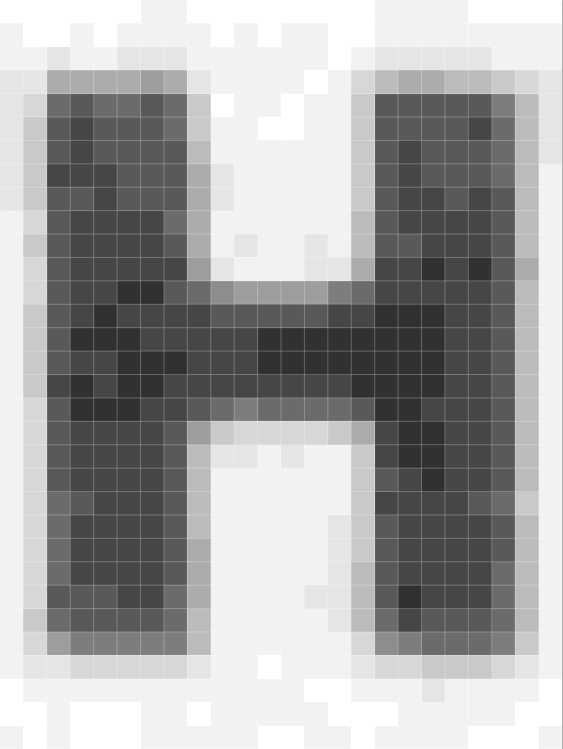
\includegraphics[width=0.05\textwidth]{assets/binarization/gray3_big.png}
        &
        
\includegraphics[width=0.05\textwidth]{assets/binarization/h25t.png}
        &
        
\includegraphics[width=0.05\textwidth]{assets/binarization/h38t.png}
        &
        
\includegraphics[width=0.05\textwidth]{assets/binarization/h50t.png}
        &
        
\includegraphics[width=0.05\textwidth]{assets/binarization/h63t.png}
        &
        
\includegraphics[width=0.05\textwidth]{assets/binarization/h75t.png}
        &
        
\includegraphics[width=0.05\textwidth]{assets/binarization/h88t.png}
        \\

        % histogramas

        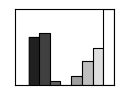
\includegraphics[scale=0.4]{assets/binarization/3bit_hist.png}
        &
        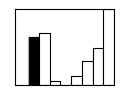
\includegraphics[scale=0.4]{assets/binarization/13hist.png}
        &
        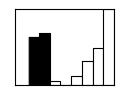
\includegraphics[scale=0.4]{assets/binarization/25hist.png}
        &
        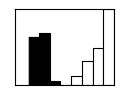
\includegraphics[scale=0.4]{assets/binarization/50hist.png}
        &
        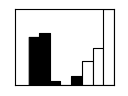
\includegraphics[scale=0.4]{assets/binarization/63hist.png}
        &
        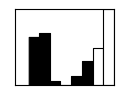
\includegraphics[scale=0.4]{assets/binarization/75hist.png}
        &
        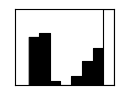
\includegraphics[scale=0.4]{assets/binarization/88hist.png}

        \\
        % peso do background
        $w_\mathbb{B}$ & 0.1931 & 0.4015 & 0.4179 & 0.4532 & 0.5479 & 0.6969 \\

        % média do background
        $\mu_\mathbb{B}$ & 34.00 & 51.64 & 53.61 & 61.37 & 83.08 & 112.56 \\

        % variância do background
        $\sigma^{2}_{\mathbb{B}}$ & 7.27 & 288.58 & 372.94 & 1054.08 & 3128.03 & 5656.37 \\

        % peso do foreground
        $w_{\mathbb{F}}$ & 0.80 & 0.59 & 0.58 & 0.54 & 0.45 & 0.30 \\

        % média do foreground
        $\mu_{\mathbb{F}}$ & 184.87 & 225.55 & 229.03 & 233.95 & 243.79 & 255.0 \\

        % variância do foreground
        $\sigma^{2}_{\mathbb{F}}$ & 5799.89 & 1409.01 & 1006.11 & 673.10 & 255.43 & 0.0 \\

        % variância intra-classe
        $\sigma^{2}_{w}$ & 21495165144 & 967521582 & 512693389 & 595067475 & 4269882800 & 17660993341 \\

        \label{tab:otsu}
      \end{tabular}
    \end{table}
    \end{center}

    Como podemos notar, para $t = 50\%$ atingimos o menor valor de $\sigma^{2}_{w} \approx 512693389$. Neste caso o limiar coincide com o único vale no histograma, porém isto nem sempre será válido. Algumas imagens não possuem vales bem definidos. Este algoritmo não se baseia no formato do histograma mas sim na coesão intra classe e na separabilidade das classes.

    \begin{figure*}[htb]
      \begin{center}
        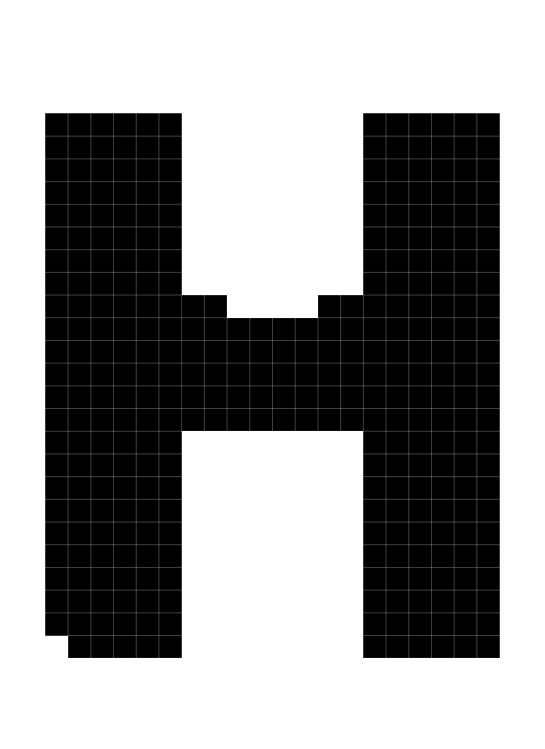
\includegraphics[width=0.5\textwidth]{assets/binarization/bin_big.png}
        \end{center}
      \caption{Imagem binarizada com $t = 50\%.$}
      \label{fig:letrah_bin}
    \end{figure*}

    Uma desvantagem de utilizar este algoritmo é a influência da média de todo os pixels da imagem. Isto pode fazer com que o limiar ótimo para a página toda não seja o mesmo que o de dentro de uma janela.

    % 
    % Usei o imagemagick para criar uma imagem em tons de cinza com a quantidade de níveis desejado, usando o seguinte comando
    % 
    % convert -type Grayscale -depth 3 h8rgb.png h_3grayscale.png
    % 
    % Posteriormente gerei imagens com threshold em diferentes níveis
    % 
    % convert -threshold 60% h_3grayscale.png h60t.png
    % 
    % o comando identify -verbose mostra o histograma
    % 
    % Usei o gráfico do site http://www.labbookpages.co.uk/software/imgProc/otsuThreshold.html como exemplo
    % 
    % binarizado com ../otsuthresh -g save h_3grayscale.png bin.gif
    % 

      %% \subsubsection{Álgebra booleana}

      %% Definições básicas até minimização de expressões.

      %% \subsubsection{Probabilidade}

      %% \begin{itemize}
      %%   \item Espaço amostral, eventos, etc
      %%   \item FDP
      %%   \item Probabilidade conjunta e condicional
      %%   \item Variável aleatória
      %%   \item Experança estatística
      %%   \item Processo estacionário
      %% \end{itemize}

%\bibliographystyle{alpha}
{\small 
\bibliographystyle{unsrt} % (uses file "plain.bst")
\bibliography{myrefs}   % expects file "myrefs.bib"
}

\end{document}
